%-------------------------------------------------------------------------------
%   CHAPTER 3 - METHODOLOGY
%-------------------------------------------------------------------------------

\section{Судалгааны арга зүй}

\subsection{Хөгжүүлэлтийн арга зүй}
Програм хангамжийг хөгжүүлэхдээ **Agile** арга зүйг, тэр дундаа **Scrum** фреймворкийг ашигласан. Энэ нь төслийг бага хэмжээний, удирдах боломжтой хэсгүүдэд (Sprints) хувааж, тогтмол хугацаанд үр дүнг гаргах, хэрэглэгчийн санал хүсэлтэд тулгуурлан сайжруулалт хийх боломжийг олгодог.

\subsection{Системийн шинжилгээ}
Системийн шаардлагыг тодорхойлохдоо хэрэглэгчийн түүх (User Stories) болон хэрэглээний тохиолдол (Use Cases) аргуудыг ашигласан.

\subsubsection{Хэрэглэгчийн ангилал}
\begin{itemize}
    \item \textbf{Захиалагч (Customer):} Бараа захиалах дэлгүүр, ресторан, хувь хүн.
    \item \textbf{Нийлүүлэгч (Supplier):} Бараа нийлүүлэгч компани, бөөний төв.
    \item \textbf{Хүргэгч (Courier):} Барааг хүргэх үүрэгтэй ажилтан.
    \item \textbf{Админ (Admin):} Системийн хэвийн үйл ажиллагааг хангах, хэрэглэгчдийг удирдах.
\end{itemize}

\subsubsection{Функциональ шаардлага}
Систем нь дараах үндсэн функциональ шаардлагуудыг хангасан байна.

\begin{longtable}{|p{1.5cm}|p{4cm}|p{7cm}|}
\caption{Функциональ шаардлагууд} \label{tab:func_req} \\
\hline
\textbf{ID} & \textbf{Шаардлага} & \textbf{Тайлбар} \\
\hline
\endfirsthead
\hline
\textbf{ID} & \textbf{Шаардлага} & \textbf{Тайлбар} \\
\hline
\endhead
\hline
\endfoot
\hline
\endlastfoot

FR-01 & Бүртгэл ба Нэвтрэх & Хэрэглэгч утасны дугаар болон имэйлээр бүртгүүлэх, нэвтрэх боломжтой байх. \\
\hline
FR-02 & Бараа хайх & Захиалагч барааг нэр, төрөл, үнээр шүүж хайх. \\
\hline
FR-03 & Сагс удирдах & Барааг сагсанд нэмэх, тоо хэмжээг өөрчлөх, хасах. \\
\hline
FR-04 & Захиалга үүсгэх & Сагсан дахь барааг баталгаажуулж захиалга илгээх. \\
\hline
FR-05 & Захиалга хянах & Захиалгын төлөвийг (Pending, Confirmed, Delivering, Delivered) бодит цагт харах. \\
\hline
FR-06 & Захиалга удирдах & Нийлүүлэгч ирсэн захиалгыг хүлээн авах эсвэл цуцлах. \\
\hline
FR-07 & Хүргэлт хуваарилах & Нийлүүлэгч захиалгыг хүргэгчид хуваарилах. \\
\hline
FR-08 & e-POD бүртгэх & Хүргэгч барааг хүлээлгэн өгөхдөө зураг авч, гарын үсэг зуруулж баталгаажуулах. \\
\hline
\end{longtable}

\subsubsection{Функциональ бус шаардлага}
\begin{itemize}
    \item \textbf{Найдвартай байдал:} Систем нь 99.9\%-ийн ажиллах хугацаатай (uptime) байна.
    \item \textbf{Аюулгүй байдал:} Хэрэглэгчийн нууц үг шифрлэгдсэн байх, өгөгдлийн хандалт нь дүрэмд (Security Rules) захирагдах.
    \item \textbf{Гүйцэтгэл:} Үйлдлийн хариу өгөх хугацаа 2 секундээс хэтрэхгүй байх.
    \item \textbf{Өргөтгөх боломж:} Хэрэглэгчийн тоо нэмэгдэхэд систем гацахгүй ажиллах (Scalability).
\end{itemize}

\subsubsection{Хэрэглээний тохиолдлын диаграмм (Use Case Diagram)}
Системийн үндсэн хэрэглэгчид болон тэдгээрийн үйлдэл, харилцан хамаарлыг дараах диаграммаар харуулав.

\begin{figure}[h]
    \centering
    \begin{tikzpicture}[scale=0.8, every node/.style={scale=0.8}]
        % Actors
        \node[draw, circle, minimum size=1cm] (customer) at (0, 4) {Customer};
        \node[draw, circle, minimum size=1cm] (supplier) at (10, 4) {Supplier};
        \node[draw, circle, minimum size=1cm] (courier) at (5, -2) {Courier};

        % Use Cases
        \node[draw, ellipse] (login) at (5, 6) {Login/Register};
        \node[draw, ellipse] (order) at (2, 2) {Place Order};
        \node[draw, ellipse] (manage) at (8, 2) {Manage Products};
        \node[draw, ellipse] (accept) at (8, 0) {Accept Order};
        \node[draw, ellipse] (deliver) at (5, 0) {Deliver Order};
        \node[draw, ellipse] (track) at (2, 0) {Track Order};

        % Connections
        \draw (customer) -- (login);
        \draw (supplier) -- (login);
        \draw (courier) -- (login);
        
        \draw (customer) -- (order);
        \draw (customer) -- (track);
        
        \draw (supplier) -- (manage);
        \draw (supplier) -- (accept);
        
        \draw (courier) -- (deliver);
        \draw (courier) -- (track);
    \end{tikzpicture}
    \caption{Системийн Use Case диаграмм}
    \label{fig:usecase}
\end{figure}

\subsubsection{Үйл ажиллагааны диаграмм (Activity Diagram)}
Захиалга үүсгэхээс эхлээд хүргэгдэх хүртэлх үйл явцыг Activity диаграммаар дүрслэв.

\begin{figure}[h]
    \centering
    \begin{tikzpicture}[node distance=1.5cm, auto]
        % Nodes
        \node[draw, rounded corners] (start) {Start};
        \node[draw, rectangle, below of=start] (place) {Place Order};
        \node[draw, diamond, below of=place, aspect=2] (check) {Stock Available?};
        \node[draw, rectangle, left of=check, node distance=3cm] (cancel) {Cancel Order};
        \node[draw, rectangle, below of=check, node distance=2cm] (notify) {Notify Supplier};
        \node[draw, rectangle, below of=notify] (prepare) {Prepare Order};
        \node[draw, rectangle, below of=prepare] (assign) {Assign Courier};
        \node[draw, rectangle, below of=assign] (deliver) {Deliver to Customer};
        \node[draw, rounded corners, below of=deliver] (end) {End};

        % Edges
        \draw[->] (start) -- (place);
        \draw[->] (place) -- (check);
        \draw[->] (check) -- node {No} (cancel);
        \draw[->] (check) -- node {Yes} (notify);
        \draw[->] (notify) -- (prepare);
        \draw[->] (prepare) -- (assign);
        \draw[->] (assign) -- (deliver);
        \draw[->] (deliver) -- (end);
        \draw[->] (cancel) |- (end);
    \end{tikzpicture}
    \caption{Захиалгын үйл явцын Activity диаграмм}
    \label{fig:activity}
\end{figure}

\subsection{Системийн архитектур}
"Tdelivery" систем нь орчин үеийн **Serverless** архитектурт суурилсан. Энэ нь сервер талын дэд бүтцийг удирдах шаардлагагүйгээр, зөвхөн бизнесийн логик болон код бичихэд төвлөрөх боломжийг олгодог.

\begin{figure}[h]
    \centering
    \begin{tikzpicture}[node distance=2cm]
        \node[draw, rectangle, minimum width=2.5cm, minimum height=1cm] (app) {Mobile App (React Native)};
        \node[draw, rectangle, right of=app, node distance=4cm] (auth) {Firebase Auth};
        \node[draw, rectangle, below of=auth] (firestore) {Cloud Firestore};
        \node[draw, rectangle, below of=firestore] (functions) {Cloud Functions};
        \node[draw, cylinder, shape border rotate=90, draw, minimum height=1cm, minimum width=1.5cm, right of=firestore, node distance=4cm] (db) {NoSQL DB};

        \draw[<->] (app) -- (auth);
        \draw[<->] (app) -- (firestore);
        \draw[<->] (firestore) -- (functions);
        \draw[<->] (firestore) -- (db);
    \end{tikzpicture}
    \caption{Системийн архитектур}
    \label{fig:architecture}
\end{figure}

\subsubsection{Технологийн сонголт}
\begin{itemize}
    \item \textbf{Frontend (Mobile App):} React Native (Expo SDK). Кросс-платформ хөгжүүлэлт хийхэд тохиромжтой, хурдан, өндөр гүйцэтгэлтэй.
    \item \textbf{Backend (BaaS):} Google Firebase.
        \begin{itemize}
            \item \textbf{Authentication:} Хэрэглэгчийн бүртгэл, нэвтрэх эрх.
            \item \textbf{Firestore:} NoSQL өгөгдлийн сан.
            \item \textbf{Cloud Functions:} Сервер талын логик.
            \item \textbf{Storage:} Зураг, файл хадгалах.
        \end{itemize}
\end{itemize}

\subsection{Өгөгдлийн сангийн зохиомж (ERD)}
Систем нь NoSQL төрлийн Cloud Firestore өгөгдлийн санг ашиглана. Өгөгдлийн хамаарлыг ER диаграммаар харуулав.

\begin{figure}[h]
    \centering
    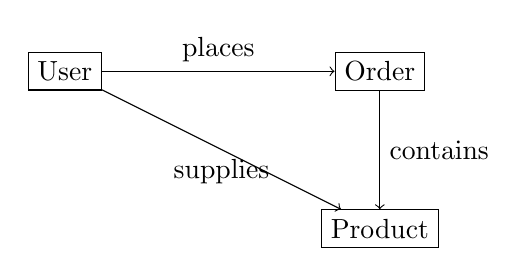
\begin{tikzpicture}[node distance=2cm]
        \node[draw, rectangle] (user) {User};
        \node[draw, rectangle, right of=user, node distance=4cm] (order) {Order};
        \node[draw, rectangle, below of=order] (product) {Product};
        
        \draw[->] (user) -- node[above] {places} (order);
        \draw[->] (user) -- node[below] {supplies} (product);
        \draw[->] (order) -- node[right] {contains} (product);
    \end{tikzpicture}
    \caption{Өгөгдлийн сангийн ER диаграмм (Хялбаршуулсан)}
    \label{fig:erd}
\end{figure}

\subsubsection{Өгөгдлийн сангийн бүтэц (Schema)}
Firestore нь схемгүй (schemaless) боловч өгөгдлийн бүрэн бүтэн байдлыг хангахын тулд дараах бүтцийг баримтална.

\textbf{1. Users Collection}
\begin{itemize}
    \item \texttt{uid} (String): Хэрэглэгчийн ID (PK)
    \item \texttt{email} (String): Имэйл хаяг
    \item \texttt{role} (String): 'customer' | 'supplier' | 'courier'
    \item \texttt{displayName} (String): Нэр
    \item \texttt{phoneNumber} (String): Утасны дугаар
    \item \texttt{address} (Map): Хаягийн мэдээлэл (lat, lng, street)
\end{itemize}

\textbf{2. Products Collection}
\begin{itemize}
    \item \texttt{id} (String): Бүтээгдэхүүний ID (PK)
    \item \texttt{supplierId} (String): Нийлүүлэгчийн ID (FK)
    \item \texttt{name} (String): Нэр
    \item \texttt{price} (Number): Үнэ
    \item \texttt{stock} (Number): Үлдэгдэл
    \item \texttt{imageUrl} (String): Зургийн зам
    \item \texttt{category} (String): Ангилал
\end{itemize}

\textbf{3. Orders Collection}
\begin{itemize}
    \item \texttt{id} (String): Захиалгын ID (PK)
    \item \texttt{customerId} (String): Захиалагчийн ID (FK)
    \item \texttt{supplierId} (String): Нийлүүлэгчийн ID (FK)
    \item \texttt{items} (Array): Захиалсан бараанууд [{productId, quantity, price}]
    \item \texttt{totalAmount} (Number): Нийт дүн
    \item \texttt{status} (String): 'pending' | 'confirmed' | 'delivering' | 'delivered' | 'cancelled'
    \item \texttt{createdAt} (Timestamp): Үүсгэсэн огноо
\end{itemize}

\subsection{Алгоритм ба Логик шийдэл}
Системийн үр ашигтай ажиллагааг хангахын тулд хэд хэдэн алгоритм, логик шийдлүүдийг хэрэгжүүлсэн.

\subsubsection{Атомик Денормализаци (Atomic Denormalization)}
NoSQL өгөгдлийн санд өгөгдлийг унших хурдыг нэмэгдүүлэхийн тулд денормализаци хийх нь түгээмэл байдаг. Гэвч өгөгдлийн зөрчил үүсэх эрсдэлтэй. Үүнийг шийдэхийн тулд Firestore Transaction ашиглан "Атомик Денормализаци" аргыг хэрэгжүүлсэн.

\subsubsection{Бодит цагийн захиалгын удирдлага}
Захиалгын төлөв өөрчлөгдөх бүрт хэрэглэгчдэд шууд харагдах ёстой. Үүний тулд \texttt{onSnapshot} сонсогч (listener) ашигласан.

\subsection{Тестлэлт}
Системийн чанарыг баталгаажуулахын тулд Unit Testing, Integration Testing, User Acceptance Testing (UAT) зэрэг аргуудыг ашигласан.

\vfill
